%% point absorbers %%

 \begin{outline}
    \1 ITM point absorbers
     \begin{figure}[H]
            \centering
            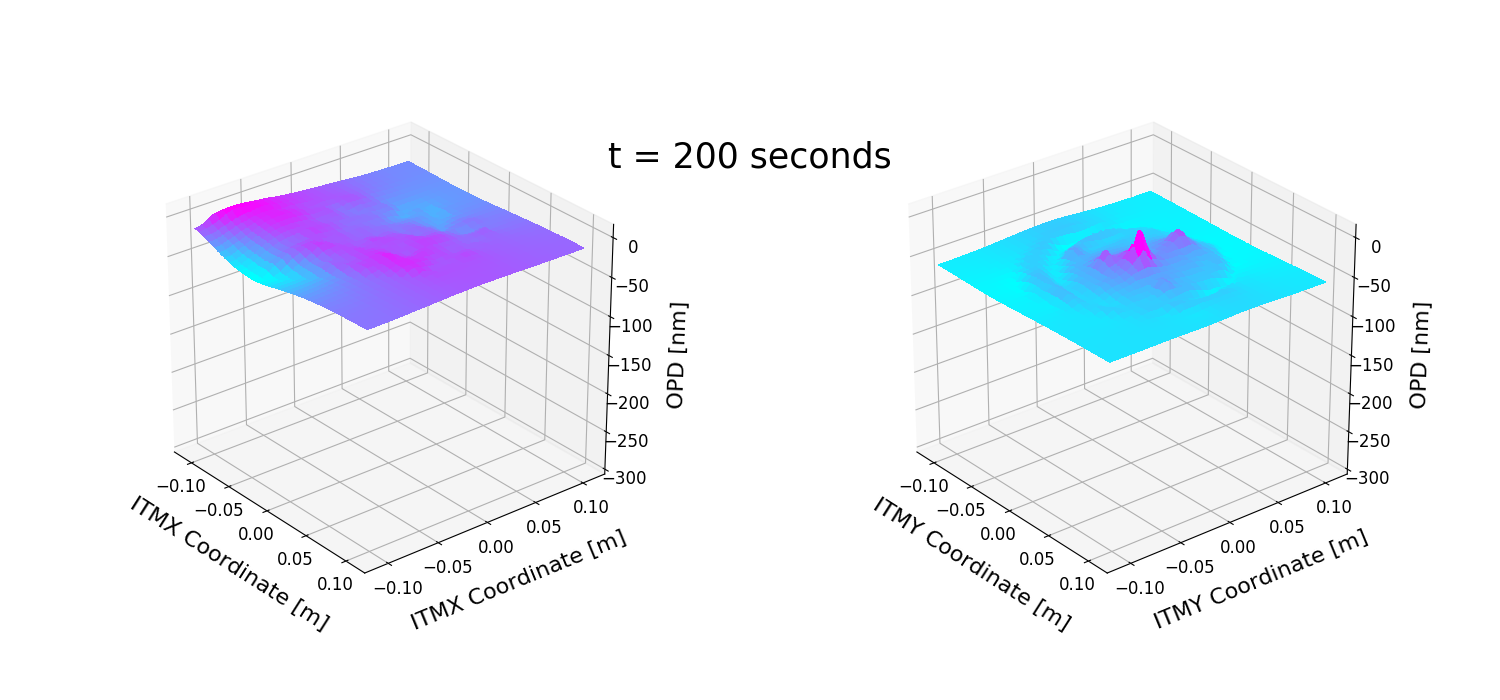
\includegraphics[width=.6\textwidth]{1231726400_3d_200dur_30W_ITM.png}
            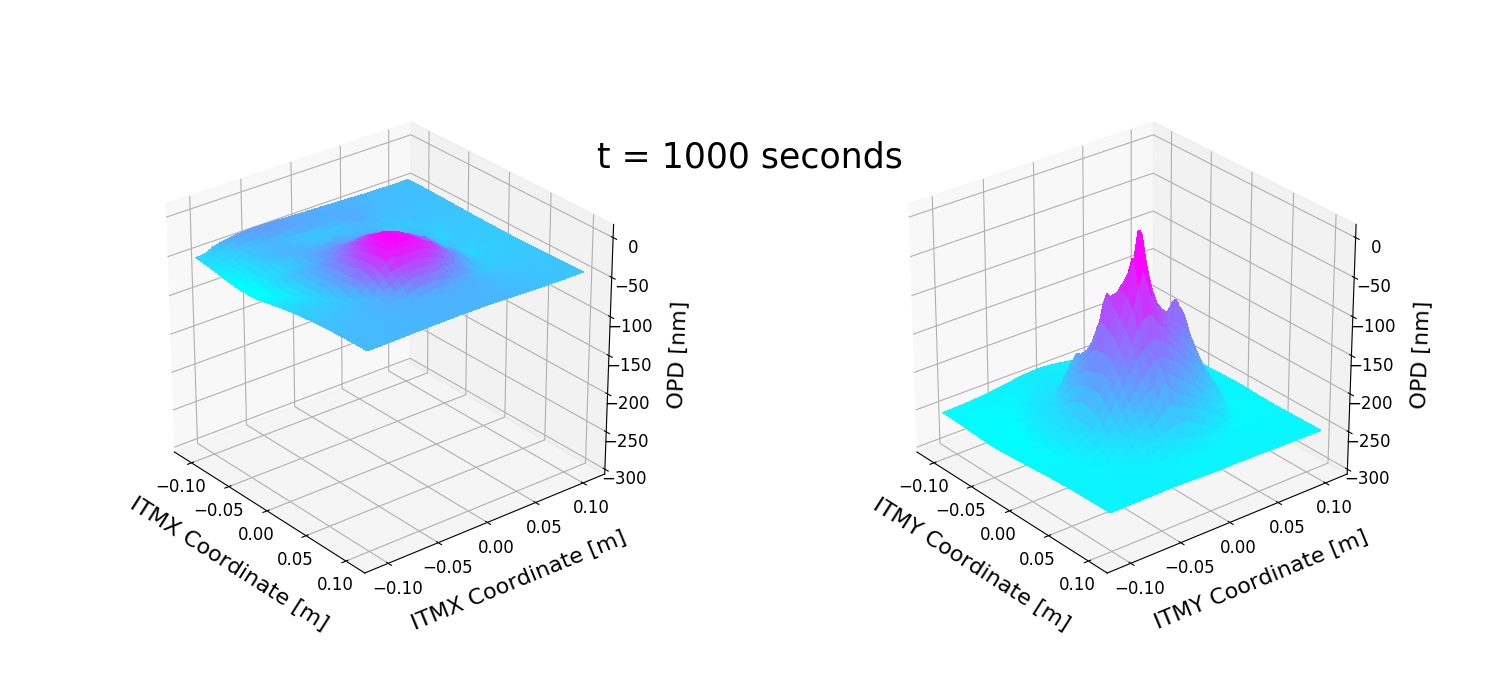
\includegraphics[width=.6\textwidth]{1231726400_3d_1000dur_30W_ITM.png}
            \caption{Comparision between the ITMX and ITMY HWS. PC: Thomas Vo}
      \end{figure}
        
    \2 ETM point absorbers
        \3 \href{https://alog.ligo-wa.caltech.edu/aLOG/index.php?callRep=45727}{alog 45727}
        
        \3 \href{https://alog.ligo-wa.caltech.edu/aLOG/index.php?callRep=44952}{first post}
    \2 Hurts contrast see Figure 3
    \2 Fast reduction in PRG and sideband buildup when increasing power to ifo
        \3 Time constant measurements
        \3 Dan's finesse simulation (\href{https://dcc.ligo.org/DocDB/0158/G1900090/002/20190116_tcs_call.pdf}{G1900090})
    \2 Scattering of the carrier into higher order modes in the arm cavities
        \3 Hiro's model
            \4 \href{https://dcc.ligo.org/DocDB/0158/G1900257/001/G1900257-v1.pdf}{Scattering of arm power to (n+m) = 7} 
    \1 Mode matching of the carrier from the Power Recycling cavities to the arms
        \2 Gabriele's models
            \3 \href{https://alog.ligo-wa.caltech.edu/aLOG/index.php?callRep=47027}{9 MHz (n+m)=9 transmission}
        \2 Hiro's model
 \end{outline}